%-------------------------------------------------------------------------------
%                            BAB II
%               TINJAUAN PUSTAKA DAN DASAR TEORI
%-------------------------------------------------------------------------------

\chapter{TINJAUAN KEPUSTAKAAN}

\section{Laser-Induced Breakdown Spectroscopy (LIBS)}
\label{sec:libs_intro}

\textit{Laser-Induced Breakdown Spectroscopy} (LIBS) adalah teknik analisis kimia yang menggunakan pulsa laser untuk menghasilkan plasma pada permukaan material, menghasilkan cahaya dengan panjang gelombang tertentu yang mencerminkan komposisi kimia material \citep{Cremers2013}. LIBS menawarkan analisis cepat, tidak merusak sampel, dan dapat digunakan untuk berbagai material, seperti logam, mineral, atau serat optik, sehingga cocok untuk penelitian di bidang fisika dan kimia \citep{Miziolek2006}. Bagian ini menjelaskan pengenalan LIBS, cara kerjanya, cara kerja laser, ilustrasi pemompaan laser, dan komponen alat yang digunakan, dengan diagram dan tabel untuk memudahkan pemahaman.

\subsection{Prinsip LIBS}
\label{subsec:libs_principles}

LIBS bekerja dengan menembakkan pulsa laser berenergi tinggi ke permukaan material, menyebabkan material menguap dan membentuk plasma. Plasma ini mengandung atom dan ion yang tereksitasi, yang memancarkan cahaya saat elektron berpindah ke tingkat energi yang lebih rendah. Cahaya ini memiliki panjang gelombang spesifik yang menunjukkan jenis elemen dalam material, seperti besi, karbon, atau dopan erbium pada serat optik \citep{Singh2007}. Cahaya yang dipancarkan dianalisis untuk mengidentifikasi elemen dalam sampel.
\begin{figure}[h]
    \centering
    \includegraphics[width=0.8\textwidth]{images/libs-plasma.pdf}
    \caption{Proses ablasi laser dalam LIBS \citep{harmon-2021}}
    \label{fig:laser_ablation}
\end{figure}


Proses kerja LIBS meliputi tahapan berikut:
\begin{enumerate}
    \item \textbf{Penyinaran dan Ablasi Laser}: Pulsa laser difokuskan ke permukaan material, menyebabkan material menguap melalui proses ablasi, menghasilkan uap material \citep{Cremers2013}.
    \item \textbf{Pembentukan Plasma}: Energi laser menghasilkan plasma yang mengandung atom dan ion tereksitasi \citep{Miziolek2006}.
    \item \textbf{Emisi Cahaya}: Atom dan ion dalam plasma memancarkan cahaya dengan panjang gelombang spesifik.
    \item \textbf{Analisis Spektrum}: Cahaya dikumpulkan dan dianalisis menggunakan alat khusus untuk mengidentifikasi elemen berdasarkan panjang gelombangnya.
\end{enumerate}
Proses ablasi laser, sebagai tahap awal, divisualisasikan pada Gambar~\ref{fig:laser_ablation}, yang menunjukkan bagaimana laser menguapkan material untuk memulai pembentukan plasma.



\subsection{Komponen Alat LIBS}
\label{subsec:libs_setup}

\begin{figure}[H]
    \begin{center}
        \includegraphics[width=0.8\textwidth]{images/LIBS-SKEMA.pdf}
        \caption{Diagram sistem LIBS \citep{Cremers2013}}
        \label{fig:libs_setup}
    \end{center}
\end{figure}

Sistem LIBS terdiri dari beberapa komponen utama yang bekerja bersama untuk menghasilkan dan menganalisis spektrum, seperti ditunjukkan pada Gambar~\ref{fig:libs_setup}:
\begin{enumerate}
    \item \textbf{Laser}: Sumber laser, seperti Nd:YAG dengan panjang gelombang 1064 nm, menghasilkan pulsa berenergi tinggi untuk menguapkan material. Pulsa ini biasanya berdurasi sangat singkat (nanodetik) \citep{Cremers2013}.
    \item \textbf{Lensa Optik}: Lensa memfokuskan pulsa laser ke titik kecil pada sampel dan mengumpulkan cahaya yang dipancarkan dari plasma untuk diteruskan ke alat analisis \citep{Miziolek2006}.
    \item \textbf{Spektrometer}: Alat ini memisahkan cahaya menjadi panjang gelombangnya, menghasilkan spektrum yang menunjukkan garis-garis emisi elemen. Spektrometer jenis Czerny-Turner sering digunakan karena resolusinya yang baik \citep{Singh2007}.
    \item \textbf{Detektor}: Detektor seperti CCD (Charge-Coupled Device) atau ICCD (Intensified CCD) merekam intensitas cahaya. ICCD dapat mengatur waktu pengukuran untuk meningkatkan kualitas spektrum \citep{Cremers2013}.
    \item \textbf{Komputer}: Mengendalikan laser, merekam data spektrum, dan membandingkannya dengan basis data, seperti NIST, untuk mengidentifikasi elemen dalam sampel \citep{Kramida2023}.
\end{enumerate}
Untuk memperjelas fungsi masing-masing komponen, Tabel~\ref{tab:libs_components} merangkum komponen utama sistem LIBS beserta peranannya dalam analisis spektral.

\begin{table}[H]
\centering
\caption{Komponen Utama Sistem LIBS dan Fungsinya}
\label{tab:libs_components}
\begin{tabularx}{\textwidth}{>{\raggedright\arraybackslash}X>{\raggedright\arraybackslash}X}
\toprule
\textbf{Komponen} & \textbf{Fungsi} \\
\midrule
Laser (misalnya, Nd:YAG) & Menghasilkan pulsa berenergi tinggi untuk menguapkan material dan membentuk plasma \citep{Cremers2013}. \\
Lensa Optik & Memfokuskan laser ke sampel dan mengumpulkan cahaya yang dipancarkan dari plasma \citep{Miziolek2006}. \\
Spektrometer (misalnya, Czerny-Turner) & Memisahkan cahaya menjadi panjang gelombang untuk menghasilkan spektrum emisi \citep{Singh2007}. \\
Detektor (CCD atau ICCD) & Merekam intensitas cahaya untuk analisis spektrum; ICCD meningkatkan kualitas data dengan pengaturan waktu \citep{Cremers2013}. \\
Komputer & Mengendalikan laser, merekam spektrum, dan mengidentifikasi elemen dengan basis data seperti NIST \citep{Kramida2023}. \\
\bottomrule
\end{tabularx}
\end{table}
\subsection{Database NIST untuk Spektrum LIBS}
\label{subsec:nist_database}

\textit{National Institute of Standards and Technology} (NIST) menyediakan \textit{Atomic Spectra Database} (ASD) sebagai sumber data spektral untuk LIBS \citep{Kramida2023}. ASD mencakup lebih dari 180.000 garis spektral dan 90.000 tingkat energi untuk 99 elemen, dengan rentang panjang gelombang 0,4~\AA{} hingga 20.000~\si{\micro\meter}, mendukung identifikasi elemen dalam plasma LIBS. Antarmuka khusus LIBS pada ASD memungkinkan perhitungan spektrum dalam kondisi \textit{Local Thermodynamic Equilibrium} (LTE) berdasarkan suhu dan densitas elektron, menggunakan persamaan Saha dan Boltzmann untuk memodelkan intensitas garis emisi. Data ini divalidasi secara kritis, relevan untuk analisis material di berbagai aplikasi, seperti eksplorasi planet dan industri \citep{Kramida2022}. Tabel~\ref{tab:nist_features} merangkum fitur utama ASD untuk LIBS.

\begin{table}[H]
\centering
\caption{Fitur Utama NIST ASD untuk LIBS}
\label{tab:nist_features}
\begin{tabularx}{\textwidth}{>{\raggedright\arraybackslash}X>{\raggedright\arraybackslash}X}
\toprule
\textbf{Fitur} & \textbf{Deskripsi} \\
\midrule
Data Garis Spektral & $>180.000$ garis, 73.000 dengan probabilitas transisi \citep{Kramida2023}. \\
Rentang Spektral & 0,4~\AA{} -- 20.000~\si{\micro\meter} \citep{Kramida2023}. \\
Antarmuka LIBS & Pemodelan spektrum LTE berdasarkan suhu dan densitas elektron \citep{Kramida2023}. \\
Cakupan Elemen & 99 elemen dengan transisi diamati \citep{Kramida2023}. \\
Akses & \textit{Online} di \url{https://physics.nist.gov/asd} \citep{Kramida2023}. \\
\bottomrule
\end{tabularx}
\end{table}
\section{Kuantum Emisi Spektral}
\subsection{Prinsip Dasar}

Spektroskopi memanfaatkan emisi atau penyerapan foton untuk menganalisis komposisi material, dengan aplikasi seperti \textit{Laser-Induced Breakdown Spectroscopy} (LIBS) yang mengukur panjang gelombang emisi untuk mengidentifikasi unsur dalam plasma \citep{CremersRadzemski2013}. Eksitasi atom oleh energi eksternal, seperti laser, menghasilkan emisi foton yang mencerminkan struktur energi atom. Hukum Planck menghubungkan energi foton dengan frekuensinya melalui
\begin{equation}
E = h\nu, \label{eq:planck}
\end{equation}
di mana \( h = 4.1357 \times 10^{-15} \, \text{eV·s} \) adalah konstanta Planck dan \( \nu \) adalah frekuensi. Dengan hubungan \( \nu = c/\lambda \), di mana \( c = 2.99792458 \times 10^8 \, \text{m/s} \), energi foton dapat dinyatakan sebagai \( E = hc/\lambda \), dengan \( hc \approx 1239.84 \, \text{eV·nm} \). Hukum ini mendasari kuantifikasi energi transisi dalam spektroskopi \citep{Beiser1992}.

Formula Rydberg menggambarkan panjang gelombang emisi dari transisi elektronik antar tingkat energi, dengan bentuk
\begin{equation}
\frac{1}{\lambda} = R_\infty \left( \frac{1}{n_f^2} - \frac{1}{n_i^2} \right), \quad R_\infty = 1.0973731568 \times 10^7 \, \text{m}^{-1}, \label{eq:rydberg}
\end{equation}
di mana \( n_f \) dan \( n_i \) adalah nomor kuantum utama (\( n_i > n_f \)). Formula ini berlaku untuk atom hidrogenoid, seperti hidrogen, He\(^+\), atau Li\(^{2+}\), dengan nilai \( R_\infty \) yang sedikit disesuaikan untuk atom non-hidrogen karena efek koreksi massa inti (\textit{reduced mass correction}). Transisi antar tingkat energi menghasilkan garis spektral spesifik yang diukur dalam spektroskopi untuk identifikasi unsur \citep{Griffiths2005}.

Transisi elektronik dalam atom diatur oleh aturan seleksi, yang menentukan transisi yang diizinkan berdasarkan perubahan bilangan kuantum dan memengaruhi intensitas garis spektral dalam spektroskopi. Aturan seleksi utama meliputi \( \Delta l = \pm 1 \), \( \Delta m_l = 0, \pm 1 \), dan \( \Delta S = 0 \), yang memastikan konservasi momentum sudut orbital (\( l \)), komponen proyeksi momentum sudut (\( m_l \)), dan spin total (\( S \)). Aturan ini berasal dari sifat simetri fungsi gelombang atom dan interaksi elektromagnetik antara elektron dan foton, yang dijelaskan melalui elemen matriks dipol
\begin{equation}
P \propto |\langle \psi_k | \vec{\mu} | \psi_i \rangle|^2, \label{eq:dipole}
\end{equation}
dengan \( \psi_i \) dan \( \psi_k \) sebagai keadaan awal dan akhir, serta \( \hat{\mu} \) sebagai operator momen dipol. Transisi yang memenuhi aturan seleksi memiliki probabilitas tinggi, menghasilkan garis spektral yang kuat, sedangkan transisi yang melanggar aturan (transisi terlarang) memiliki probabilitas rendah dan menghasilkan garis spektral lemah, yang terkadang masih terdeteksi dalam kondisi tertentu, seperti pada atom berat. Untuk atom hidrogen, aturan seleksi memungkinkan transisi seri Balmer (misalnya, H\(\alpha\), H\(\beta\), H\(\gamma\)), yang menghasilkan garis spektral kuat dalam rentang tampak, penting untuk aplikasi seperti LIBS. 
\par Kopling spin-orbit, yang timbul dari interaksi antara momentum sudut orbital dan spin elektron, menyebabkan pemisahan tingkat energi menjadi sub-level, dikenal sebagai struktur halus (\textit{fine structure}). Efek ini lebih signifikan pada atom dengan nomor atom tinggi, seperti natrium atau merkuri, karena pengaruh relativistik yang meningkatkan interaksi spin-orbit. Sebagai contoh, pada natrium, garis D (sekitar 589 nm) menunjukkan pemisahan struktur halus akibat kopling spin-orbit, yang terdeteksi sebagai dua garis spektral berdekatan dalam spektroskopi. Dalam LIBS, aturan seleksi membantu memprediksi garis spektral yang dominan, seperti H\(\alpha\) untuk hidrogen atau garis natrium untuk atom alkali, memungkinkan analisis kuantitatif komposisi plasma. Transisi terlarang, seperti pelanggaran \( \Delta S = 0 \), dapat terjadi pada atom berat karena kopling spin-orbit yang kuat, menghasilkan garis spektral lemah yang tetap relevan dalam analisis spektral presisi tinggi \citep{Griffiths2005, CremersRadzemski2013, Demtroder2010}.
\subsection{Transisi Elektronik Atom Hidrogen}

Dalam atom hidrogen, energi elektron pada tingkat kuantum \( n \) diberikan oleh
\begin{equation}
E_n = -\frac{13.6}{n^2} \, \text{eV}, \quad n \in \mathbb{Z}^+, \label{eq:energy_hydrogen}
\end{equation}
dan selisih energi untuk transisi emisi dari \( n_i \) ke \( n_f \) (\( n_f < n_i \)) adalah
\begin{equation}
\Delta E = 13.6 \left( \frac{1}{n_f^2} - \frac{1}{n_i^2} \right) \, \text{eV}. \label{eq:deltaE}
\end{equation}
Seri Balmer (\( n_f = 2 \), \( n_i = 3, 4, 5 \)) menghasilkan garis spektral dalam rentang tampak, yang kritis untuk spektroskopi LIBS dalam mendeteksi hidrogen dalam plasma \citep{CremersRadzemski2013}. Menggunakan formula Rydberg (\ref{eq:rydberg}), panjang gelombang untuk seri Balmer dihitung sebagai berikut:
\begin{itemize}
    \item H\(\alpha\) (\( n_i = 3 \to n_f = 2 \)):
    \[
    \frac{1}{\lambda} = 1.0973731568 \times 10^7 \left( \frac{1}{2^2} - \frac{1}{3^2} \right), \quad \lambda \approx 656.28 \, \text{nm}.
    \]
    \item H\(\beta\) (\( n_i = 4 \to n_f = 2 \)):
    \[
    \frac{1}{\lambda} = 1.0973731568 \times 10^7 \left( \frac{1}{2^2} - \frac{1}{4^2} \right), \quad \lambda \approx 486.13 \, \text{nm}.
    \]
    \item H\(\gamma\) (\( n_i = 5 \to n_f = 2 \)):
    \[
    \frac{1}{\lambda} = 1.0973731568 \times 10^7 \left( \frac{1}{2^2} - \frac{1}{5^2} \right), \quad \lambda \approx 434.05 \, \text{nm}.
    \]
\end{itemize}
Data ini divalidasi dengan basis data NIST \citep{Kramida2023}. Aturan seleksi (\( \Delta l = \pm 1 \), \( \Delta m_l = 0, \pm 1 \), \( \Delta S = 0 \)) memastikan transisi seri Balmer diizinkan, menghasilkan garis spektral yang kuat dalam rentang tampak, dengan garis H\(\alpha\) pada 656.28 nm sebagai indikator utama keberadaan hidrogen dalam LIBS \citep{CremersRadzemski2013}.

Diagram Grotrian memvisualisasikan tingkat energi dan transisi yang diizinkan, seperti seri Balmer, memungkinkan analisis transisi elektronik dalam plasma \citep{Mason2015}. Diagram ini ditunjukkan pada Gambar~\ref{fig:grotrian}, dengan tingkat energi dihitung menggunakan persamaan (\ref{eq:energy_hydrogen}) dan transisi emisi digambarkan sebagai panah ke bawah untuk H\(\alpha\), H\(\beta\), dan H\(\gamma\).

\begin{figure}[h]
    \begin{center}
        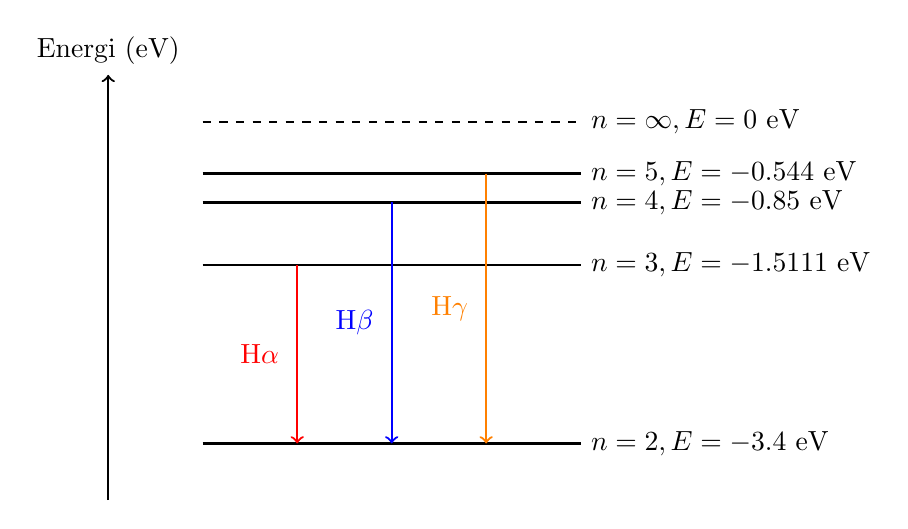
\begin{tikzpicture}[scale=1.2]
            % Sumbu energi (vertikal)
            \draw[->, thick] (0,-4) -- (0,0.5) node[above] {Energi (eV)};
            
            % Tingkat energi
            \draw[thick] (1,-3.4) -- (5,-3.4) node[right] {$n=2, E=-3.4$ eV};
            \draw[thick] (1,-1.5111) -- (5,-1.5111) node[right] {$n=3, E=-1.5111$ eV};
            \draw[thick] (1,-0.85) -- (5,-0.85) node[right] {$n=4, E=-0.85$ eV};
            \draw[thick] (1,-0.544) -- (5,-0.544) node[right] {$n=5, E=-0.544$ eV};
            \draw[thick, dashed] (1,0) -- (5,0) node[right] {$n=\infty, E=0$ eV};
            
            % Transisi emisi (panah ke bawah)
            \draw[->, thick, red] (2,-1.5111) -- (2,-3.4) node[midway, left=0.1cm] {H\(\alpha\)};
            \draw[->, thick, blue] (3,-0.85) -- (3,-3.4) node[midway, left=0.1cm] {H\(\beta\)};
            \draw[->, thick, orange] (4,-0.544) -- (4,-3.4) node[midway, left=0.1cm] {H\(\gamma\)};
        \end{tikzpicture}
        \caption{Diagram Grotrian untuk atom hidrogen pada seri Balmer dengan \(\lambda_{\text{H}\alpha} = 656.28 \, \text{nm}\), \(\lambda_{\text{H}\beta} = 486.13 \, \text{nm}\), \(\lambda_{\text{H}\gamma} = 434.05 \, \text{nm}\). \label{fig:grotrian}}
    \end{center}
\end{figure}
\section{Distrbusi Populasi dan Ionisasi dalam Plasma LIBS}

\subsection{Distribusi Boltzmann}
Dalam plasma LIBS, populasi atom pada tingkat energi tertentu bergantung pada suhu plasma. Dalam kesetimbangan termal lokal, distribusi Boltzmann menentukan probabilitas pada tingkat energi ke-\( i \), yaitu \( P_i \), sebagai:
\begin{equation}
P_i \propto g_i e^{-\frac{E_i}{k_B T}}, \label{eq:boltzmann_propto}
\end{equation}
dimana \( g_i \) adalah faktor degenerasi, \( E_i \) adalah energi tingkat ke-\( i \), dan \( k_B = 8.617 \times 10^{-5} \, \text{eV / K} \) adalah konstanta Boltzmann. Kemudian, jika \( N \) adalah populasi atom, maka fraksi populasi relatif untuk tingkat energi ke-\( i \) adalah:
\begin{equation}
N_i = \frac{N g_i e^{-\frac{E_i}{k_B T}}}{Z}, \label{eq:boltzmann1}
\end{equation}
dan fungsi partisi \( Z \) didefinisikan sebagai:
\begin{equation}
Z = \sum_i g_i e^{-\frac{E_i}{k_B T}}, \label{eq:partition}
\end{equation}
Fungsi partisi memastikan normalisasi sehingga \( \sum_i N_i = N \). Persamaan ini bergantung pada suhu \( T \) dan sifat atom seperti energi \( E_i \) dan degenerasi \( g_i \) yang dapat diakses dari \textit{National Institute of Standards and Technology} (NIST) \citep{Pathria2011,Rybicki1985}.

\subsection{Intensitas Garis Spektral}
Intensitas garis spektral \( I_{ik} \) dihasilkan dari emisi spontan saat atom bertransisi dari tingkat energi atas \( E_k \) ke tingkat energi bawah \( E_i \) (\( E_i < E_k \)). Probabilitas emisi spontan per satuan waktu diberikan oleh \( A_{ki} \). Daya total yang dihasilkan adalah:
\begin{equation}
P_{k} = N_k A_{ki} h \nu_{ki}, \label{eq:power}
\end{equation}
Intensitas garis spektral \( I_{ik} \) dihasilkan dari emisi spontan saat atom bertransisi dari tingkat energi atas \( E_k \) ke tingkat energi bawah \( E_i \) (\( E_k > E_i \)). Energi foton yang dipancarkan diberikan oleh:
\begin{equation}
h \nu_{ik} = E_k - E_i,
\end{equation}
dimana \( \nu_{ik} = \frac{E_k - E_i}{h} \) adalah frekuensi foton, dan \( \lambda_{ik} = \frac{c}{\nu_{ik}} = \frac{h c}{E_k - E_i} \) adalah panjang gelombang terkait, dengan \( h \nu_{ik} = \frac{h c}{\lambda_{ik}} \) dan \( h c \approx 1239.84 \, \text{eV·nm} \). Probabilitas emisi spontan per satuan waktu ditentukan oleh koefisien Einstein \( A_{ik} \) \citep{Rybicki1985}. Daya total yang dihasilkan dari transisi ini adalah:
\begin{equation}
P_k = N_k A_{ik} h \nu_{ik}, \label{eq:power}
\end{equation}
dimana \( N_k \) adalah populasi atom pada tingkat energi \( E_k \), dihitung menggunakan distribusi Boltzmann [Persamaan~\eqref{eq:boltzmann1}]. Intensitas \( I_{ik} \), yaitu daya per satuan sudut ruang dalam sudut solider \( 4\pi \) steradian, diberikan oleh:
\begin{equation}
I_{ik} = \frac{P_k}{4\pi} = \frac{N_k A_{ik} h \nu_{ik}}{4\pi}. \label{eq:intensity}
\end{equation}

Dengan mensubstitusi \( N_k \) dari Persamaan~\eqref{eq:boltzmann1}, dimana \( g_k \) adalah faktor degenerasi tingkat \( E_k \), \( k_B = \SI{8.617e-5}{\electronvolt\per\kelvin} \) adalah konstanta Boltzmann, \( T \) adalah suhu plasma, dan \( Z \) adalah fungsi partisi [Persamaan~\eqref{eq:partition}], intensitas menjadi:
\begin{equation}
I_{ik} = \frac{N g_k A_{ik} h \nu_{ik} e^{-\frac{E_k}{k_B T}}}{4\pi Z}. \label{eq:intensity_full}
\end{equation}

Dimana \( h \nu_{ik} \) dan \( 4\pi \) dapat diabaikan untuk perhitungan intensitas relatif yang dinormalisasi. Persamaan ini akan memfokuskan pada ketergantungan intensitas terhadap suhu plasma dan parameter spesifik transisi (\( g_k \), \( A_{ik} \), \( E_k \)). Dengan demikian, intensitas relatif dinyatakan sebagai:
\begin{equation}
I_{ik} \propto \frac{N g_k A_{ik} e^{-\frac{E_k}{k_B T}}}{Z}. \label{eq:intensity_relative}
\end{equation}

dimana \( Z \) dihitung untuk setiap tingkat energi transisi. Persamaan ini digunakan untuk menghitung intensitas relatif pada setiap panjang gelombang \( \lambda_{ik} \), yang penting untuk memodelkan spektrum \citep{Rybicki1985,Draine2011,Mason2015}.

\subsection{Persamaan Saha untuk Populasi Ion}

Persamaan Saha digunakan untuk menghitung rasio ionisasi \( \frac{n_{i+1} n_e}{n_i} \) berdasarkan suhu plasma \( T \), densitas elektron \( n_e \), dan energi ionisasi atom. Persamaan ini menggambarkan keseimbangan ionisasi:
\[
A_i \leftrightarrow A_i^+ + e^-.
\]
Untuk menurunkannya, kita mulai dengan fungsi partisi, yang merepresentasikan jumlah keadaan kuantum yang dapat diakses oleh partikel dalam kesetimbangan termal \citep{Pathria2011}.

Fungsi partisi total untuk setiap partikel (atom netral \( A_i \), ion \( A_i^+ \), atau elektron \( e^- \)) terdiri dari komponen translasional dan internal. Fungsi partisi translasional dihitung secara umum untuk partikel bebas dengan massa \( m \) dalam volume \( V \):
\begin{equation}
Z_{\text{trans}} = \frac{1}{h^3} \int e^{-p^2/(2m k_B T)} \, d^3q \, d^3p, \label{eq:partition_trans}
\end{equation}
dimana \( h \) adalah konstanta Planck, \( k_B = \SI{8.617e-5}{\electronvolt\per\kelvin} \) adalah konstanta Boltzmann, dan \( T \) adalah suhu plasma. Faktor \( 1/h^3 \) menormalkan ruang fase untuk setiap keadaan kuantum. Integral over posisi menghasilkan:
\begin{equation}
\int d^3q = V. \label{eq:integral_position}
\end{equation}
Integral over momentum, menggunakan koordinat bola dan substitusi \( u = p^2/(2m k_B T) \), adalah:
\begin{equation}
\int e^{-p^2/(2m k_B T)} \, d^3p = \left( 2\pi m k_B T \right)^{3/2}. \label{eq:integral_momentum}
\end{equation}
Substitusi ke dalam Persamaan~\eqref{eq:partition_trans} menghasilkan:
\begin{equation}
Z_{\text{trans}} = V \left( \frac{2\pi m k_B T}{h^2} \right)^{3/2}. \label{eq:partition_trans_final}
\end{equation}

Untuk atom netral (\( A_i \)) dengan massa \( m_i \):
\begin{equation}
Z_{i,\text{trans}} = V \left( \frac{2\pi m_i k_B T}{h^2} \right)^{3/2}. \label{eq:partition_trans_neutral}
\end{equation}
Untuk ion (\( A_i^+ \)) dengan massa \( m_{i+1} \approx m_i \):
\begin{equation}
Z_{i+1,\text{trans}} = V \left( \frac{2\pi m_{i+1} k_B T}{h^2} \right)^{3/2}. \label{eq:partition_trans_ion}
\end{equation}
Fungsi partisi internal mencakup keadaan energi elektronik:
\begin{equation}
Z_{\text{int}} = \sum_m g_m e^{-E_m/(k_B T)}, \label{eq:partition_internal}
\end{equation}
dimana \( g_m \) adalah faktor degenerasi keadaan dengan energi \( E_m \). Pada suhu LIBS (10.000–30.000 K), hanya keadaan dasar yang dominan, sehingga fungsi partisi internal untuk atom netral dan ion masing-masing adalah:
\[
Z_{i,\text{int}} \approx g_i, \quad Z_{i+1,\text{int}} \approx g_{i+1},
\]
dimana \( g_i \) dan \( g_{i+1} \) adalah degenerasi keadaan dasar. Fungsi partisi total untuk atom netral dan ion adalah:
\begin{equation}
Z_i = Z_{i,\text{int}} Z_{i,\text{trans}} = g_i \left( \frac{2\pi m_i k_B T}{h^2} \right)^{3/2} V, \quad Z_{i+1} = g_{i+1} \left( \frac{2\pi m_{i+1} k_B T}{h^2} \right)^{3/2} V. \label{eq:partition_total}
\end{equation}

Untuk elektron, yang merupakan fermion dengan spin-1/2, fungsi partisi harus mempertimbangkan statistik Fermi-Dirac:
\begin{equation}
f(E) = \frac{1}{e^{(E - \mu)/(k_B T)} + 1}, \label{eq:fermi_dirac}
\end{equation}
dimana \( \mu \) adalah potensial kimia. Dalam plasma LIBS pada suhu 10.000–30.000 K, densitas elektron rendah, sehingga plasma bersifat non-degenerasi (\( e^{(E - \mu)/(k_B T)} \gg 1 \)). Pada batas ini, distribusi Fermi-Dirac mendekati distribusi Maxwell-Boltzmann:
\begin{equation}
f(E) \approx e^{-(E - \mu)/(k_B T)}, \label{eq:fermi_dirac_approx}
\end{equation}
memungkinkan pendekatan klasik untuk menghitung fungsi partisi translasional elektron \citep{Pathria2011}. Dengan massa elektron \( m_e \), fungsi partisi translasional elektron adalah:
\begin{equation}
Z_{e,\text{trans}} = V \left( \frac{2\pi m_e k_B T}{h^2} \right)^{3/2}, \label{eq:partition_trans_electron}
\end{equation}
sesuai dengan Persamaan~\eqref{eq:partition_trans_final}. Elektron memiliki dua keadaan spin (\( m_s = \pm 1/2 \)), memberikan faktor degenerasi spin \( g_e = 2 \). Oleh karena itu, fungsi partisi total untuk elektron adalah:
\begin{equation}
Z_e = g_e Z_{e,\text{trans}} = 2 \left( \frac{2\pi m_e k_B T}{h^2} \right)^{3/2} V. \label{eq:partition_electron}
\end{equation}

Untuk menurunkan persamaan Saha, kita mempertimbangkan keseimbangan termal reaksi ionisasi \( A_i \leftrightarrow A_i^+ + e^- \). Rasio densitas dalam kesetimbangan termal diberikan oleh:
\begin{equation}
\frac{n_{i+1} n_e}{n_i} = \frac{Z_{i+1} Z_e}{Z_i} e^{-\frac{E_{xi}}{k_B T}}, \label{eq:saha_initial}
\end{equation}
dimana \( E_{xi} \) adalah energi ionisasi atom, diperoleh dari database NIST. Substitusi fungsi partisi dari Persamaan~\eqref{eq:partition_total} dan~\eqref{eq:partition_electron}:
\begin{equation}
\frac{n_{i+1} n_e}{n_i} = \frac{g_{i+1} \left( \frac{2\pi m_{i+1} k_B T}{h^2} \right)^{3/2} V \cdot 2 \left( \frac{2\pi m_e k_B T}{h^2} \right)^{3/2} V}{g_i \left( \frac{2\pi m_i k_B T}{h^2} \right)^{3/2} V} e^{-\frac{E_{xi}}{k_B T}}. \label{eq:saha_substitution}
\end{equation}
Karena \( m_i \approx m_{i+1} \), faktor massa dan volume membatalkan, sehingga:
\begin{equation}
\frac{n_{i+1} n_e}{n_i} = \frac{2 g_{i+1}}{g_i} \left( \frac{2\pi m_e k_B T}{h^2} \right)^{3/2} e^{-\frac{E_{xi}}{k_B T}}. \label{eq:saha_final}
\end{equation}
Dengan \( Z_{i,\text{int}} = g_i \) dan \( Z_{i+1,\text{int}} = g_{i+1} \), persamaan Saha dapat ditulis sebagai:
\begin{equation}
\frac{n_{i+1}}{n_i} = \frac{\frac{N_{i+1}}{V}} {\frac{N_{i}}{V}}= \frac{N_{i+1}} {N_{i}} = \frac{2Z_{i+1,\text{int}}}{N_eZ_{i,\text{int}}} \left( \frac{2\pi m_e k_B T}{h^2} \right)^{3/2} e^{-\frac{E_{xi}}{k_B T}}. \label{eq:saha_final_int}
\end{equation}

Persamaan ini kemudian digunakan untuk menghitung rasio ionisasi dengan memasukkan suhu plasma \( T \), densitas elektron \( n_e \), dan energi ionisasi \( E_{xi} \). Konstanta-konstanta memiliki asal-usul fisik: faktor 2 dari degenerasi spin elektron, \( Z_{i+1,\text{int}}/Z_{i,\text{int}} \) dari rasio degenerasi keadaan dasar, \( \left( \frac{2\pi m_e k_B T}{h^2} \right)^{3/2} \) dari densitas keadaan translasional elektron, dan \( e^{-\frac{E_{xi}}{k_B T}} \) dari probabilitas ionisasi. Persamaan Saha berlaku untuk plasma non-degenerasi dalam LIBS, tetapi memerlukan modifikasi untuk plasma padat, seperti dalam kondisi ekstrem \citep{Chandrasekhar1939}.

Untuk memastikan plasma berada dalam kondisi \textit{Local Thermodynamic Equilibrium} (selanjutnya disebut LTE), kriteria McWhirter menetapkan batas minimum densitas elektron untuk LTE sebagai \citep{McWhirter1965}:
\begin{equation}
n_e \geq 1.6 \times 10^{12} T^{1/2} \Delta E^3 \, \text{cm}^{-3}, \label{eq:mcwhirter}
\end{equation}
dimana \( T \) adalah suhu dalam eV dan \( \Delta E \) adalah perbedaan energi antar level dalam eV. Kondisi ini memvalidasi asumsi distribusi Boltzmann, yang mendasari interpretasi data spektral temporal.

\section{Profil Garis Spektral dalam LIBS}

Dalam \textit{Laser-Induced Breakdown Spectroscopy} (LIBS), profil garis spektral merupakan alat penting untuk menentukan parameter plasma, seperti suhu (\( T \)), densitas elektron (\( n_e \)), dan komposisi elemen. Profil garis dihasilkan dari transisi elektronik atom atau ion dalam plasma, yang dipengaruhi oleh mekanisme pelebaran seperti efek Doppler, tekanan (termasuk pelebaran Stark), dan efek instrumental. Mekanisme ini menghasilkan profil Gaussian, Lorentzian, atau kombinasi keduanya (Voigt), yang memengaruhi intensitas garis, resolusi spektral, dan akurasi pengukuran parameter plasma \citep{Demtroder2010,Griem1997}. Bagian berikut menjelaskan profil garis ini, hubungan fisiknya dengan kondisi plasma.

\subsection{Pelebaran Doppler dan Profil Gaussian}
Efek Doppler, yang disebabkan oleh gerakan termal atom atau ion dalam plasma LIBS, menghasilkan pelebaran garis spektral dengan profil Gaussian:
\begin{equation}
G(\lambda) = \frac{1}{\sqrt{2\pi \sigma^2}} \exp\left(-\frac{(\lambda - \lambda_0)^2}{2\sigma^2}\right), \label{eq:gaussian}
\end{equation}
dimana \( \lambda_0 \) adalah panjang gelombang pusat transisi, dan \( \sigma \) adalah lebar setengah maksimum (HWHM) yang diberikan oleh:
\begin{equation}
\sigma = \frac{\lambda_0}{c} \sqrt{\frac{k_B T}{m}}, \label{eq:sigma_doppler}
\end{equation}
dengan \( c = \SI{2.998e8}{\meter\per\second} \) sebagai kecepatan cahaya, \( k_B = \SI{8.617e-5}{\electronvolt\per\kelvin} \) sebagai konstanta Boltzmann, \( T \) sebagai suhu plasma (dalam kelvin), dan \( m \) sebagai massa atom atau ion \citep{Demtroder2010}. Lebar Doppler (\( \sigma \)) sebanding dengan \( \sqrt{T/m} \), mencerminkan distribusi kecepatan Maxwell-Boltzmann dari partikel dalam plasma. Dalam LIBS, efek Doppler dominan pada tekanan rendah (< 1 mbar) dan suhu tinggi (10.000–30.000 K), memungkinkan estimasi suhu plasma melalui pemasangan profil Gaussian \citep{Miziolek2006}.

\subsection{Pelebaran Tekanan dan Profil Lorentzian}
Pelebaran tekanan, yang diakibatkan oleh tumbukan antara atom/ion pemancar dengan partikel lain (elektron, ion, atau atom netral) dalam plasma LIBS, menghasilkan profil Lorentzian:
\begin{equation}
L(\lambda) = \frac{\Gamma / 2\pi}{(\lambda - \lambda_0)^2 + (\Gamma / 2)^2}, \label{eq:lorentzian}
\end{equation}
dimana \( \Gamma \) adalah lebar penuh setengah maksimum (FWHM) yang bergantung pada densitas plasma. Dalam LIBS, pelebaran Stark, akibat interaksi dengan elektron dan ion, sering kali mendominasi \( \Gamma \). Lebar Stark dapat diaproksimasi sebagai:
\begin{equation}
\Gamma \approx 2w \left( \frac{n_e}{10^{16}} \right), \label{eq:stark_broadening}
\end{equation}
dimana \( w \) adalah parameter pelebaran Stark (dalam nm) untuk transisi spesifik, dan \( n_e \) adalah densitas elektron (dalam \( \text{cm}^{-3} \)) \citep{Griem1997,Konjevic1999}. Untuk transisi hidrogen seperti H\(\alpha\) (garis spektral hidrogen pada 656.3 nm), \( w \approx 0.1 \, \text{nm} \) pada \( T \approx 10.000 \, \text{K} \) dan \( n_e \approx 10^{16} \, \text{cm}^{-3} \). Pelebaran tekanan signifikan pada densitas elektron tinggi (\( n_e > 10^{15} \, \text{cm}^{-3} \)), memengaruhi intensitas sayap garis dan akurasi pengukuran distribusi Boltzmann \citep{Aragon2008}.

\subsection{Profil Voigt untuk Analisis Spektrum}
Profil Voigt adalah konvolusi dari profil Gaussian (efek Doppler dan instrumental) dan Lorentzian (efek tekanan/Stark):
\begin{equation}
V(\lambda; \Gamma, \sigma) = \int_{-\infty}^{\infty} G(\lambda - \lambda') L(\lambda') \, d\lambda', \label{eq:voigt}
\end{equation}
dimana \( \sigma \) dan \( \Gamma \) masing-masing adalah lebar Gaussian dan Lorentzian. Profil Voigt menggabungkan efek Doppler, yang dominan di pusat garis, dengan efek tekanan/Stark, yang dominan di sayap garis, menjadikannya model akurat untuk garis spektral dalam plasma LIBS \citep{Griem1997}. Dalam  LIBS, profil Voigt digunakan untuk memodelkan bentuk garis spektral, memungkinkan ekstraksi parameter plasma seperti suhu (\( T \)) dari komponen Gaussian dan densitas elektron (\( n_e \)) dari komponen Lorentzian. Selain itu, profil Voigt kritis untuk menghitung intensitas garis yang digunakan dalam analisis distribusi Boltzmann untuk menentukan populasi tingkat energi \citep{Miziolek2006,Aragon2008}.

\subsection{Efek Fisik Profil Garis pada Analisis Spektral}
Mekanisme pelebaran garis memengaruhi analisis spektral dalam LIBS melalui hubungan kuantitatif dengan parameter plasma. Tabel~\ref{tab:broadening_effects} merangkum mekanisme pelebaran, profil garis terkait, parameter fisik yang memengaruhinya, dan dampaknya pada pengukuran spektral.

\begin{table}[h]
\centering
\caption{Mekanisme Pelebaran Garis Spektral dalam LIBS}
\label{tab:broadening_effects}
\begin{tabularx}{\textwidth}{XXXX}
\toprule
\textbf{Mekanisme Pelebaran} & \textbf{Profil Garis} & \textbf{Parameter Fisik} & \textbf{Dampak pada Analisis Spektral} \\
\midrule
Doppler & Gaussian & Suhu (\( T \)), massa atom (\( m \)) & Estimasi \( T \) melalui lebar \( \sigma \); memengaruhi resolusi spektral \citep{Demtroder2010}. \\
Stark & Lorentzian & Densitas elektron (\( n_e \)), suhu & Pengukuran \( n_e \) melalui lebar \( \Gamma \); dominan pada \( n_e > 10^{15} \, \si{\per\cubic\centi\meter} \) \citep{Griem1997,Konjevic1999}. \\
Tekanan (van der Waals) & Lorentzian & Densitas atom netral, tekanan & Memengaruhi sayap garis pada tekanan tinggi \citep{Konjevic1999}. \\
Instrumental & Gaussian & Resolusi spektrometer & Mengurangi akurasi lebar garis dan resolusi spektral \citep{Miziolek2006}. \\
Voigt (Konvolusi) & Voigt & \( T \), \( n_e \), resolusi & Model akurat untuk \( T \) dan \( n_e \); kunci untuk distribusi Boltzmann \citep{Aragon2008}. \\
\bottomrule
\end{tabularx}
\end{table}

Efek fisik dari pelebaran garis dalam LIBS meliputi:
\begin{itemize}
  \item \textbf{Suhu Plasma}: Lebar Doppler (\( \sigma \)) sebanding dengan \( \sqrt{T/m} \), memungkinkan pengukuran suhu plasma melalui pemasangan profil Gaussian. Untuk atom hidrogen pada \( T = 10.000 \, \text{K} \), \( \sigma \approx 0.01 \, \text{nm} \) untuk H\(\alpha\) \citep{Demtroder2010}.
  \item \textbf{Densitas Elektron}: Lebar Stark (\( \Gamma \)) berkorelasi dengan \( n_e \), memungkinkan diagnosis densitas elektron melalui pemasangan profil Lorentzian atau Voigt \citep{Griem1997,Konjevic1999}.
  \item \textbf{Intensitas Garis dan Distribusi Boltzmann}: Luas puncak spektral, yang dipengaruhi oleh profil Voigt, menentukan intensitas garis yang digunakan untuk menghitung rasio populasi tingkat energi dalam distribusi Boltzmann [Persamaan~\eqref{eq:boltzmann1}] \citep{Miziolek2006}.
  \item \textbf{Resolusi Spektral}: Pelebaran instrumental dan Doppler dapat mengaburkan garis spektral yang berdekatan, mengurangi kemampuan untuk membedakan transisi \citep{Aragon2008}.
\end{itemize}

Kemudian profil Voigt dihitung menggunakan algoritma numerik, seperti aproksimasi Humlíček, untuk memodelkan garis spektral dengan akurasi tinggi sambil meminimalkan biaya komputasi \citep{Griem1997}. Pendekatan ini memungkinkan analisis kuantitatif parameter plasma dan komposisi elemen dengan memisahkan kontribusi Gaussian dan Lorentzian melalui dek convolusi \citep{Aragon2008}.

\section{Pembelajaran Mendalam: Pemodelan Deret Waktu Berbasis \textit{Transformer}}
\label{sec:transformer_informer}

Pemodelan deret waktu adalah inti dari analisis data sekuensial, seperti prediksi cuaca, analisis data spektral, dan berbagai aplikasi berbasis deret waktu. Tantangan utamanya adalah menangkap ketergantungan jarak jauh (\textit{long-range dependencies}) dalam urutan panjang dengan efisiensi komputasi tinggi. Pemodelan deret waktu telah berkembang dari \textit{Recurrent Neural Networks} (RNN) \citep{Bengio1994}, yang terhambat oleh masalah \textit{vanishing gradient} dan pemrosesan sekuensial \citep{Hochreiter1997}. Model seperti \textit{Long Short-Term Memory} (LSTM) dan \textit{Gated Recurrent Unit} (GRU) meningkatkan penanganan ketergantungan jarak jauh, tetapi tetap kurang efisien untuk deret waktu sangat panjang \citep{Hochreiter1997}. \textit{Transformer}, diperkenalkan oleh \citet{Vaswani2017}, merevolusi pemrosesan deret waktu dengan mekanisme \textit{self-attention} yang memungkinkan pemrosesan paralel dan panjang jalur maksimum \( O(1) \). Namun, kompleksitas kuadratiknya (\( O(n^2) \)) membatasi skalabilitas untuk urutan panjang.

\begin{table}[H]
\centering
\caption{Perbandingan Karakteristik RNN dan \textit{Transformer}}
\label{tab:rnn_vs_transformer}
\begin{tabularx}{\textwidth}{>{\raggedright\arraybackslash}X>{\raggedright\arraybackslash}X>{\raggedright\arraybackslash}X}
\toprule
\textbf{Aspek} & \textbf{RNN} & \textbf{\textit{Transformer}} \\
\midrule
Proses & Rekursif, \( O(n) \) operasi sekuensial & Paralel, \( O(1) \) operasi sekuensial \\
Ketergantungan Jarak Jauh & Sulit (\textit{vanishing gradient}) & Efektif (\textit{self-attention}) \\
Kompleksitas per Lapisan & \( O(n \cdot d^2) \) & \( O(n^2 \cdot d) \) \\
Panjang Jalur Maksimum & \( O(n) \) & \( O(1) \) \\
\bottomrule
\end{tabularx}
\end{table}

\subsection{Arsitektur \textit{Transformer}}
Arsitektur \textit{Transformer} terdiri dari \textit{encoder} dan \textit{decoder}, masing-masing dengan \( N=6 \) lapisan identik, yang dirancang untuk memproses deret waktu secara paralel \citep{Vaswani2017}. Setiap lapisan \textit{encoder} memiliki dua sub-lapisan: \textit{multi-head self-attention} untuk menangkap ketergantungan temporal dan jaringan \textit{feed-forward} posisi-\textit{wise} untuk transformasi non-linear. Operasi penjumlahan (\textit{residual connection}) dan normalisasi lapisan (\textit{layer normalization}) diterapkan setelah setiap sub-lapisan:
\begin{equation}
y = x + \text{Sublayer}(x), \quad \text{LayerNorm}(y) = \gamma \cdot \frac{y - \mu}{\sqrt{\sigma^2 + \epsilon}} + \beta
\end{equation}
di mana \( x \in \mathbb{R}^{n \times 512} \) adalah input sub-lapisan (dimensi \( d_{\text{model}} = 512 \)), \(\text{Sublayer}(x)\) adalah output sub-lapisan, \( \mu \) dan \( \sigma^2 \) adalah rata-rata dan varians fitur per token, dan \( \epsilon = 10^{-5} \) mencegah pembagian nol. Parameter \( \gamma \) dan \( \beta \) memungkinkan penskalaan fleksibel. Operasi ini memastikan stabilitas pelatihan dengan mengurangi perubahan distribusi fitur, yang sangat penting untuk deret waktu multivariat seperti prediksi konsumsi energi, di mana pola temporal bervariasi. \textit{Decoder} menambahkan sub-lapisan \textit{multi-head attention} atas output \textit{encoder} dan \textit{masking} untuk sifat auto-regresif, memungkinkan peramalan deret waktu secara iteratif.

\begin{figure}[h]
    \centering
    \includegraphics[width=0.6\textwidth]{images/ModalNet-21.png}
    \caption{Arsitektur \textit{Transformer} \autocite{Vaswani2017}}
    \label{fig:transformer_architecture}
\end{figure}

\subsection{Mekanisme \textit{Attention}}
\label{sec:attention}



Mekanisme \textit{self-attention} adalah inti dari \textit{Transformer}, memungkinkan model menghitung ketergantungan antar token dalam urutan secara paralel \citep{Vaswani2017}. Menggunakan \textit{scaled dot-product attention}, setiap token direpresentasikan sebagai matriks \textit{query} (\( Q \)), \textit{key} (\( K \)), dan \textit{value} (\( V \)) dengan dimensi \( \mathbb{R}^{n \times d_k} \), di mana \( n \) adalah panjang urutan dan \( d_k = 64 \) (untuk \( h=8 \)). Skor perhatian dihitung sebagai:
\begin{equation}
\text{Score}_{ij} = \frac{(Q_i \cdot K_j)}{\sqrt{d_k}}
\end{equation}
Skor ini diskalakan oleh \( \sqrt{d_k} \) untuk mencegah nilai besar yang mengganggu \textit{softmax}, lalu dikonversi menjadi bobot perhatian:
\begin{equation}
\text{Attention}(Q, K, V) = \text{softmax}\left(\frac{QK^T}{\sqrt{d_k}}\right)V
\end{equation}
Operasi ini memiliki kompleksitas \( O(n^2 \cdot d_k) \), tetapi memungkinkan model menangkap hubungan temporal jarak jauh, seperti pola musiman dalam prediksi cuaca atau tren jangka panjang dalam konsumsi energi, tanpa ketergantungan pada pemrosesan sekuensial seperti RNN.
\begin{figure}[h]
    \centering
    \begin{subfigure}[t]{0.3\textwidth}
        \centering
        \includegraphics[width=\textwidth]{images/ModalNet-19.png}
        \caption{Mekanisme \textit{self-attention} dalam \textit{Transformer}}
        \label{fig:self_attention_a}
    \end{subfigure}
    \hfill
    \begin{subfigure}[t]{0.3\textwidth}
        \centering
        \includegraphics[width=\textwidth]{images/ModalNet-20.png}
        \caption{\textit{Scaled Dot-Product Attention}}
        \label{fig:self_attention_b}
    \end{subfigure}
    \caption{Ilustrasi mekanisme \textit{self-attention} dan \textit{scaled dot-product attention} dalam \textit{Transformer} \autocite{Vaswani2017}}
    \label{fig:self_attention_comparison}
\end{figure}
\subsection{\textit{Multi-Head Attention}}
\label{sec:multi_head_attention}

\textit{Multi-head attention} meningkatkan fleksibilitas \textit{self-attention} dengan memproyeksikan matriks \( Q \), \( K \), dan \( V \) ke \( h=8 \) ruang paralel, masing-masing dengan dimensi \( d_k = d_v = d_{\text{model}} / h = 64 \), untuk \( d_{\text{model}} = 512 \) \citep{Vaswani2017}. Setiap kepala menghitung:
\begin{equation}
\text{head}_i = \text{Attention}(Q W_i^Q, K W_i^K, V W_i^V)
\end{equation}
di mana \( W_i^Q, W_i^K, W_i^V \in \mathbb{R}^{512 \times 64} \) adalah matriks proyeksi, dan hasilnya digabungkan:
\begin{equation}
\text{MultiHead}(Q, K, V) = \text{Concat}(\text{head}_1, \ldots, \text{head}_8) W^O
\end{equation}
dengan \( W^O \in \mathbb{R}^{512 \times 512} \). Kompleksitas tetap \( O(n^2 \cdot d_{\text{model}}) \), tetapi setiap kepala menangkap pola temporal berbeda, seperti korelasi jangka pendek (misalnya, harian) dan jangka panjang (misalnya, mingguan) dalam deret waktu multivariat. Misalnya, dalam prediksi konsumsi energi, \textit{multi-head attention} dapat menghubungkan suhu harian dengan pola penggunaan listrik tahunan.

\subsection{\textit{Position-wise Feed-Forward Networks}}
\label{sec:ffn}

Setiap lapisan \textit{encoder} dan \textit{decoder} memiliki jaringan \textit{feed-forward} posisi-\textit{wise} (FFN) yang diterapkan pada setiap token secara independen (lihat Gambar~\ref{fig:transformer_architecture}) \citep{Vaswani2017}. FFN didefinisikan sebagai:
\begin{equation}
\text{FFN}(x) = \max(0, x W_1 + b_1) W_2 + b_2
\end{equation}
di mana \( x \in \mathbb{R}^{512} \), \( W_1 \in \mathbb{R}^{512 \times 2048} \), \( b_1 \in \mathbb{R}^{2048} \), \( W_2 \in \mathbb{R}^{2048 \times 512} \), dan \( b_2 \in \mathbb{R}^{512} \). Fungsi aktivasi ReLU (\(\max(0, \cdot)\)) memperkenalkan non-linearitas, memungkinkan model menangkap pola kompleks seperti anomali (misalnya, lonjakan konsumsi energi) atau perubahan tren. Kompleksitas FFN adalah \( O(n \cdot d_{\text{model}} \cdot d_{\text{ff}}) \), linier terhadap panjang urutan \( n \). Dalam deret waktu, FFN meningkatkan kapasitas representasi dengan memproses setiap titik waktu secara independen, mendukung analisis spektral atau prediksi cuaca.

\subsection{\textit{Positional Encoding}}
\label{sec:positional_encoding}

Karena \textit{Transformer} tidak memiliki rekurensi, informasi posisi token disuntikkan melalui \textit{positional encoding} (PE) \citep{Vaswani2017}. Untuk urutan dengan panjang \( n \), PE adalah matriks \( \mathbb{R}^{n \times 512} \), dihitung sebagai:
\begin{equation}
PE_{(pos, 2i)} = \sin\left(\frac{pos}{10000^{2i/512}}\right), \quad PE_{(pos, 2i+1)} = \cos\left(\frac{pos}{10000^{2i/512}}\right)
\end{equation}
di mana \( pos \) adalah indeks posisi (0 hingga \( n-1 \)), dan \( i \) adalah indeks dimensi (0 hingga 255). PE ditambahkan ke vektor input:
\begin{equation}
x_{\text{input}} = x + PE
\end{equation}
dengan \( x \in \mathbb{R}^{n \times 512} \) sebagai vektor representasi token. Fungsi sinusoid memastikan pola periodik yang mendukung generalisasi ke urutan panjang, krusial untuk peramalan deret waktu panjang seperti prediksi cuaca bulanan. Sifat ini memungkinkan model mempertahankan urutan temporal tanpa ketergantungan sekuensial.

\subsection{Kelebihan dan Keterbatasan}
\label{sec:transformer_limits}

\textit{Transformer} menawarkan keunggulan signifikan untuk pemodelan deret waktu \citep{Vaswani2017}:
\begin{enumerate}
    \item \textbf{Ketergantungan Jarak Jauh}: Panjang jalur maksimum \( O(1) \), memungkinkan model menangkap hubungan temporal seperti pola musiman tanpa batasan RNN.
    \item \textbf{Paralelisme}: Pemrosesan paralel mengurangi waktu pelatihan (12 jam pada 8 GPU P100 untuk WMT 2014).
    \item \textbf{Fleksibilitas}: Digeneralisasi ke tugas seperti analisis spektral (F1 92.7 untuk \textit{parsing}).
\end{enumerate}

Namun, keterbatasan meliputi:
\begin{enumerate}
    \item \textbf{Kompleksitas Kuadratik}: Kompleksitas waktu per lapisan adalah \( O(n^2 \cdot d) \) untuk \textit{self-attention} dan \( O(n \cdot d \cdot d_{\text{ff}}) \) untuk FFN, menghasilkan total:
    \begin{equation}
    \text{Waktu} = O(N \cdot (n^2 \cdot d + n \cdot d \cdot d_{\text{ff}}))
    \end{equation}
    Memori juga kuadratik: \( O(N \cdot n^2) \), membatasi skalabilitas untuk deret waktu panjang.
    \item \textbf{Kebutuhan Memori}: Penumpukan \( N=6 \) lapisan meningkatkan kebutuhan memori, terutama untuk \( n \) besar.
    \item \textbf{Decoding Lambat}: \textit{Dynamic decoding} auto-regresif memperlambat inferensi \citep{Zhou2021}.
\end{enumerate}
Keterbatasan ini mendorong pengembangan varian seperti \textit{Informer}, yang mengurangi kompleksitas menjadi \( O(n \cdot \log n) \) menggunakan \textit{ProbSparse self-attention}.

\section{\textit{Informer}}
\label{sec:informer}

Pemodelan deret waktu panjang (\textit{long sequence time-series forecasting}, LSTF) menghadapi tantangan dalam menangkap ketergantungan jarak jauh pada urutan dengan panjang \( n \gg 1000 \), seperti prediksi konsumsi energi atau lalu lintas \citep{Wu2021}. \textit{Transformer} \citep{Vaswani2017} unggul dalam menangkap pola musiman dan tren jangka panjang, tetapi kompleksitas kuadratiknya (\( O(n^2 \cdot d) \)) menyebabkan kebutuhan memori dan waktu komputasi yang besar. \textit{Informer}, dikembangkan oleh \citet{Zhou2021}, mengatasi keterbatasan ini dengan mengoptimalkan \textit{self-attention} menjadi \textit{ProbSparse self-attention} (kompleksitas \( O(n \cdot \ln n \cdot d) \)), menyuling fitur melalui \textit{self-attention distilling}, dan mempercepat inferensi dengan \textit{generative-style decoding}. \textit{Informer} menawarkan solusi efisien dan akurat untuk LSTF, ideal untuk penelitian empiris.

\subsection{Arsitektur \textit{Informer}}
\label{sec:informer_architecture}

\textit{Informer} mempertahankan struktur \textit{encoder-decoder} dari \textit{Transformer}, yang dioptimalkan untuk menangani LSTF \citep{Zhou2021}. \textit{Encoder} memproses urutan masukan \( \mathcal{X}^t = \{ \mathbf{x}_1^t, \ldots, \mathbf{x}_{L_x}^t \mid \mathbf{x}_i^t \in \mathbb{R}^{d_m} \} \) menggunakan \textit{ProbSparse self-attention} dan \textit{self-attention distilling}, menghasilkan representasi tersandi \( \mathbf{Z}^t \in \mathbb{R}^{L_z \times d_{\text{model}}} \), dengan \( L_z \ll L_x \). \textit{Decoder} menerima masukan \( \mathbf{X}_{\text{de}}^t \) dan menghasilkan urutan keluaran \( \mathbf{Y}^t \in \mathbb{R}^{L_y \times d_y} \) dalam satu langkah generatif, sebagaimana ditunjukkan pada persamaan berikut:
\begin{equation}
\text{Encoder: } \mathbf{X}^t \mapsto \mathbf{Z}^t, \quad \text{Decoder: } \mathbf{X}_{\text{de}}^t \mapsto \mathbf{Y}^t
\end{equation}
Kompleksitas per lapisan \textit{Informer} adalah \( O(n \cdot \ln n \cdot d) \), jauh lebih efisien dibandingkan \textit{Transformer} dengan kompleksitas \( O(n^2 \cdot d) \). Arsitektur ini mendukung aplikasi seperti prediksi konsumsi energi atau lalu lintas. Struktur keseluruhan \textit{encoder-decoder} ditunjukkan pada Gambar~\ref{fig:encoder_decoder}.

\begin{figure}[H]
    \centering
    \includegraphics[width=0.8\textwidth]{images/Encoder_Decoder_all.pdf}
    \caption{Arsitektur keseluruhan model \textit{Informer} \citep{Zhou2021}.}
    \label{fig:encoder_decoder}
\end{figure}

\subsection{\textit{ProbSparse Self-Attention}}
\label{sec:probsparse}

Mekanisme \textit{ProbSparse self-attention} dirancang untuk mengurangi kompleksitas \textit{self-attention} kanonikal dari \( O(L_Q \cdot L_K) \) menjadi \( O(L \cdot \ln L) \) untuk \( L_Q = L_K = L \) \citep{Zhou2021}. Pendekatan ini memanfaatkan distribusi skor \textit{attention} yang jarang, dengan skor \textit{attention} didefinisikan sebagai:
\begin{equation}
p(\mathbf{k}_j \mid \mathbf{q}_i) = \frac{e^{\frac{\mathbf{q}_i \mathbf{k}_j^T}{\sqrt{d}}}}{\sum_{m=1}^{L_K} e^{\frac{\mathbf{q}_i \mathbf{k}_m^T}{\sqrt{d}}}}
\end{equation}
Hanya sejumlah kecil \textit{query} dengan skor tertinggi yang dipilih, membentuk matriks \textit{query} jarang \( \overline{\mathbf{Q}} \). Proses \textit{self-attention} dihitung sebagai:
\begin{equation}
\mathcal{A}(\mathbf{Q}, \mathbf{K}, \mathbf{V}) = \text{Softmax}\left( \frac{\overline{\mathbf{Q}} \mathbf{K}^T}{\sqrt{d}} \right) \mathbf{V}
\end{equation}
Mekanisme ini memungkinkan penanganan hubungan temporal yang signifikan, seperti dalam prediksi lalu lintas, dengan efisiensi komputasi yang tinggi.

\subsection{\textit{Self-Attention Distilling}}
\label{sec:distilling}

\textit{Self-attention distilling} bertujuan untuk mengurangi dimensi temporal peta fitur pada \textit{encoder}, mengatasi \textit{memory bottleneck} \textit{Transformer} yang memiliki kompleksitas memori \( O(L^2) \) \citep{Zhou2021}. Operasi ini diterapkan antar lapisan sebagai berikut:
\begin{equation}
\mathbf{X}_{j+1}^t = \text{MaxPool}\left( \text{ELU}\left( \text{Conv1d}\left( [\mathbf{X}_j^t]_{\text{AB}} \right) \right) \right)
\end{equation}
dengan \( [\mathbf{X}_j^t]_{\text{AB}} \in \mathbb{R}^{L \times d_{\text{model}}} \) sebagai keluaran blok \textit{attention} pada lapisan ke-\( j \), \( \text{Conv1d} \) sebagai operasi konvolusi satu dimensi, dan \( \text{MaxPool} \) mengurangi dimensi temporal menjadi \( L/2 \). Kompleksitas memori menjadi:
\begin{equation}
O((2-\epsilon) \cdot L \cdot \ln L)
\end{equation}
Struktur replika tumpukan pada \textit{encoder} meningkatkan ketahanan model, mendukung analisis data deret waktu dengan dimensi besar.

\subsection{\textit{Generative-Style Decoder}}
\label{sec:decoder}

\textit{Decoder} pada \textit{Informer} menghasilkan keluaran dalam satu langkah inferensi, mengatasi keterbatasan \textit{dynamic decoding} \textit{Transformer} yang memiliki kompleksitas \( O(L_y) \) \citep{Zhou2021}. Masukan \textit{decoder} didefinisikan sebagai:
\begin{equation}
\mathbf{X}_{\text{de}}^t = \text{Concat}\left( \mathbf{X}_{\text{start}}^t, \mathbf{X}_0^t \right) \in \mathbb{R}^{(L_{\text{token}} + L_y) \times d_{\text{model}}}
\end{equation}
dengan \( \mathbf{X}_{\text{start}}^t \) sebagai \textit{start token} dan \( \mathbf{X}_0^t \) sebagai \textit{placeholder}. Mekanisme \textit{masked ProbSparse self-attention} memastikan kausalitas temporal melalui:
\begin{equation}
\text{MaskedAttention}(\mathbf{Q}, \mathbf{K}, \mathbf{V}) = \text{Softmax}\left( \frac{\overline{\mathbf{Q}} \mathbf{K}^T - M_{\text{mask}}}{\sqrt{d}} \right) \mathbf{V}
\end{equation}
Kompleksitas inferensi menjadi \( O(1) \), mendukung aplikasi real-time seperti pemantauan jaringan listrik. Proses inferensi \textit{decoder} ditunjukkan pada Gambar~\ref{fig:network_decoder}.

\begin{figure}[H]
    \centering
    \includegraphics[width=0.8\textwidth]{images/Network_Decoder.pdf}
    \caption{Proses inferensi \textit{decoder} \textit{Informer} \citep{Zhou2021}.}
    \label{fig:network_decoder}
\end{figure}

\subsection{Representasi Masukan}
\label{sec:input_representation}

Representasi masukan \textit{Informer} mengintegrasikan fitur temporal untuk menangkap dinamika deret waktu, didefinisikan sebagai:
\begin{equation}
\mathcal{X}_{\text{feed}[i]}^t = \alpha \mathbf{u}_i^t + \text{PE}_{[L_x \cdot (i-1) + 1]} + \sum_p [\text{SE}_{[L_x \cdot (i-1) + 1]}]_p
\end{equation}
dengan \( \mathbf{u}_i^t \in \mathbb{R}^{d_{\text{model}}} \) sebagai proyeksi masukan, \( \text{PE} \) sebagai \textit{positional encoding}, dan \( \text{SE} \) sebagai \textit{stamp embedding} untuk menangkap konteks waktu. Pendekatan ini mendukung analisis data multivariat, seperti dalam prediksi konsumsi energi. Proses pembentukan masukan ditunjukkan pada Gambar~\ref{fig:input_rep}.

\begin{figure}[H]
    \centering
    \includegraphics[width=0.8\textwidth]{images/Input_Rep.pdf}
    \caption{Proses pembentukan masukan model \textit{Informer} \citep{Zhou2021}.}
    \label{fig:input_rep}
\end{figure}

\subsection{Metrik Evaluasi}
\label{sec:evaluation_metrics}

Evaluasi kinerja \textit{Informer} dilakukan menggunakan metrik standar seperti \textit{Mean Squared Error} (MSE), \textit{Mean Absolute Error} (MAE), dan \textit{Root Mean Squared Error} (RMSE). \textit{MSE} didefinisikan sebagai:
\begin{equation}
\text{MSE} = \frac{1}{L_y} \sum_{i=1}^{L_y} (\mathbf{y}_i^t - \hat{\mathbf{y}}_i^t)^2
\end{equation}
yang mengukur rata-rata kuadrat selisih antara nilai prediksi \( \hat{\mathbf{y}}_i^t \) dan nilai aktual \( \mathbf{y}_i^t \). \textit{MAE} menghitung rata-rata kesalahan absolut:
\begin{equation}
\text{MAE} = \frac{1}{L_y} \sum_{i=1}^{L_y} |\mathbf{y}_i^t - \hat{\mathbf{y}}_i^t|
\end{equation}
Sedangkan \textit{RMSE} didefinisikan sebagai akar kuadrat dari \textit{MSE}:
\begin{equation}
\text{RMSE} = \sqrt{\frac{1}{L_y} \sum_{i=1}^{L_y} (\mathbf{y}_i^t - \hat{\mathbf{y}}_i^t)^2}
\end{equation}
Metrik-metrik ini memungkinkan perbandingan kinerja \textit{Informer} dengan model lain seperti \textit{Transformer} atau LSTM dalam konteks peramalan deret waktu.
